\chapter{Diskussion}\label{ch:diskussion}

Dieses Kapitel ordnet die empirischen Befunde kritisch ein und stellt ihre Tragweite für Forschung und Praxis heraus. Ausgangspunkt bilden die in Abschnitt~\ref{sec:antworten-auf-forschungsfragen} zusammengeführten Antworten auf \emph{UF1-UF4} und \emph{FF1}. Die Resultate werden in Bezug auf die Qualitätsziele aus Abschnitt~\ref{sec:qualitatsziele} interpretiert, zentrale Trade-offs (Recall vs.\ Precision) herausgearbeitet und Besonderheiten der Modellklassen gegenübergestellt. Darauf aufbauend erfolgen eine vergleichende Einordnung der Modelle und ihrer Herkunft, eine Analyse von Robustheit und Pipeline-Einflüssen sowie eine Betrachtung typischer Fehlerbilder und Grenzen. Abschließend werden Implikationen für Anwendungsszenarien und zukünftige Forschung abgeleitet.

\section{Einordnung und Interpretation}\label{sec:einordnung-und-interpretation}

Die Experimente zeigen, dass moderne \acp{LLM} \ac{DSGVO}-kritische Aktivitäten in \ac{BPMN}-Prozessen zuverlässig identifizieren können. Neun von dreizehn Modellen erreichen den angestrebten F1-Score von $\geq 0{,}80$ und erfüllen damit die in Abschnitt \ref{sec:qualitatsziele} definierten Qualitätsziele für ein wirksames Screening, das \emph{\ac{FN}} minimiert, ohne den nachfolgenden Prüfaufwand durch \emph{\ac{FP}} unverhältnismäßig zu erhöhen. Diese Priorisierung auf den \emph{Recall} ist sachlich begründet, da übersehene kritische Aktivitäten schwerwiegende rechtliche und finanzielle Konsequenzen nach sich ziehen können. Im Gegensatz dazu erhöhen \ac{FP} zwar den Prüfaufwand, führen aber nicht zu direkten Verstößen gegen die \ac{DSGVO}. Die Resultate zeigen ein heterogenes Bild: \texttt{GPT-4o} erzielt die höchste Precision mit $0{,}892$, verfehlt jedoch das Recall-Ziel. Umgekehrt erreicht \texttt{Gemma-3-27B-it} einen sehr hohen Recall von $0{,}916$, wird aber durch eine niedrige Precision von $0{,}687$ ausgebremst. Modelle wie \texttt{Qwen3-235B-A22B-Thinking-2507}, \texttt{GPT-OSS-20B} und \texttt{DeepSeek-R1-\linebreak~Distill-Qwen-14B} bieten eine ausgewogene Balance und zählen deshalb zu den Spitzenreitern. Die aggregierten Metriken in Abbildung \ref{fig:results-evaluation-metrics-comparison} und Tabelle \ref{tab:metrics-overview} bestätigen diese Einschätzung.

Ein Teil der Testfälle wurde formal als fehlerhaft gewertet, obwohl alle kritischen Aktivitäten korrekt klassifiziert worden sind. Es wurden jedoch zusätzliche Aktivitäten als kritisch markiert (\ac{FP}) und mit plausiblen Begründungen versehen. Für ein Risiko-Vorscreening ist dieses Verhalten akzeptabel und sogar wünschenswert, solange die \ac{FP}-Last den manuellen Prüfaufwand nicht unverhältnismäßig erhöht. Gleichzeitig zeigt dieses Muster die Notwendigkeit robuster Testdaten auf, die belastbare Labels enthalten: Statt Datensätze nachträglich an Modellausgaben anzupassen, empfiehlt sich für künftige Benchmarks ein Labeling mit mehreren unabhängigen Gutachtern, um subjektive Interpretationen zu minimieren und Grenzfälle klar zu definieren.
\section{Modelle im Vergleich}\label{sec:modelle-im-vergleich}

Hinsichtlich der Herkunft sind einzelne europäische Modelle wettbewerbsfähig. Dazu gehören das proprietäre \texttt{Mistral Medium 3.1} mit F1-Score $= 0{,}843$, Recall $0{,}877$ und Precision $0{,}811$ sowie das Open-Source-Modell \texttt{Mistral-Large-\linebreak~Instruct-2411} mit F1-Score $= 0{,}823$ und Recall $= 0{,}872$. Im Durchschnitt liegen jedoch internationale Modelle vorne und zeigen eine geringere Varianz und höhere Robustheit. Daraus folgt, dass die Auswahl des Modells nicht allein auf die Herkunft gestützt werden sollte, sondern dass eine ganzheitliche Bewertung der Leistungsfähigkeit, Stabilität und Transparenz beim Training und Betrieb erfolgen muss.

Beim Vergleich \emph{Open-Source vs.\ proprietär} übertreffen mehrere offene Modelle die proprietären Vertreter in F1-Score und Recall. \texttt{GPT-4o} überzeugt zwar durch eine sehr hohe Precision von $0{,}892$, verfehlt aber das Recall-Mindestziel. \texttt{Mistral Medium 3.1} bietet einen ausgewogenen Kompromiss und erfüllt alle Zielwerte, liegt aber hinter den besten Open-Source-Modellen. Für Recall-priorisierte Vorscreenings sind \texttt{Qwen3-235B-A22B-Thinking-2507}, \texttt{GPT-OSS-20B} und\linebreak\texttt{DeepSeek-R1-Distill-Qwen-14B} die stärksten Kandidaten. Diese Ergebnisse unterstreichen, dass Open-Source-Modelle in spezialisierten Aufgaben konkurrenzfähig und proprietäre Lösungen nicht zwangsläufig überlegen sind.

Mit Blick auf die \emph{Modellgröße} liegen kleine ($\leq 25B$) und große Modelle ($> 25B$) im Mittel nah beieinander. Kleine Modelle wie \texttt{GPT-OSS-20B} halten bei deutlich größeren Modellen mit oder übertreffen sie sogar. Zudem sind sie durch geringe Hardware-Anforderungen gut für On-Premises-Betrieb geeignet, was in datenschutzsensiblen Kontexten und im Hinblick auf Kosten von Vorteil ist. Die reine Parameteranzahl erweist sich damit nicht als hinreichendes Kriterium für die Modellauswahl. Vielmehr sind die Trainingsdaten, Feinabstimmung und Architektur der Modelle für ihre Leistung entscheidend. Für die Praxis bedeutet das: Die Modellauswahl sollte entlang der Zielmetrik (Recall-Priorität), dem erwarteten nachfolgenden Prüfungsaufwand (Precision) und den betrieblichen Rahmenbedingungen (Kosten, Hosting) erfolgen. Besonders wenn personenbezogene Daten verarbeitet werden, sind \ac{EU}-Hosting und On-Premises-Betrieb wichtige Kriterien, die durch kleinere, leistungsfähige Modelle erleichtert werden.
\section{Robustheit}\label{sec:robustheit}

Die Robustheit der Modelle wird anhand zweier Kriterien bewertet: der Varianz der F1-Scores über die verschiedenen Seeds und der Anzahl der Retries, die erforderlich waren, um eine formatkorrekte JSON-Antwort von den \acp{LLM} in der Klassifizierungspipeline zu erhalten. Beide Größen geben Aufschluss darüber, wie stabil ein Modell im produktiven Einsatz ist.

Abbildung \ref{fig:results-evaluation-robustness-f1-std} zeigt die Standardabweichungen der F1‑Scores über fünf unabhängige Läufe mit unterschiedlichen Seeds. Die Mehrzahl der Modelle weist Werte von deutlich unter $0{,}02$ auf. Sie liefern damit weitgehend gleiche Ergebnisse, unabhängig vom gewählten Seed, und gelten als stabil. Dazu zählen \texttt{Gemma-3-12B-it}, \texttt{Mistral-Large-Instruct-2411}, \texttt{GPT-OSS-120B} und \texttt{DeepSeek-R1-Distill-\linebreak~Qwen-14B}.

\begin{figure}[h]
    \centering
    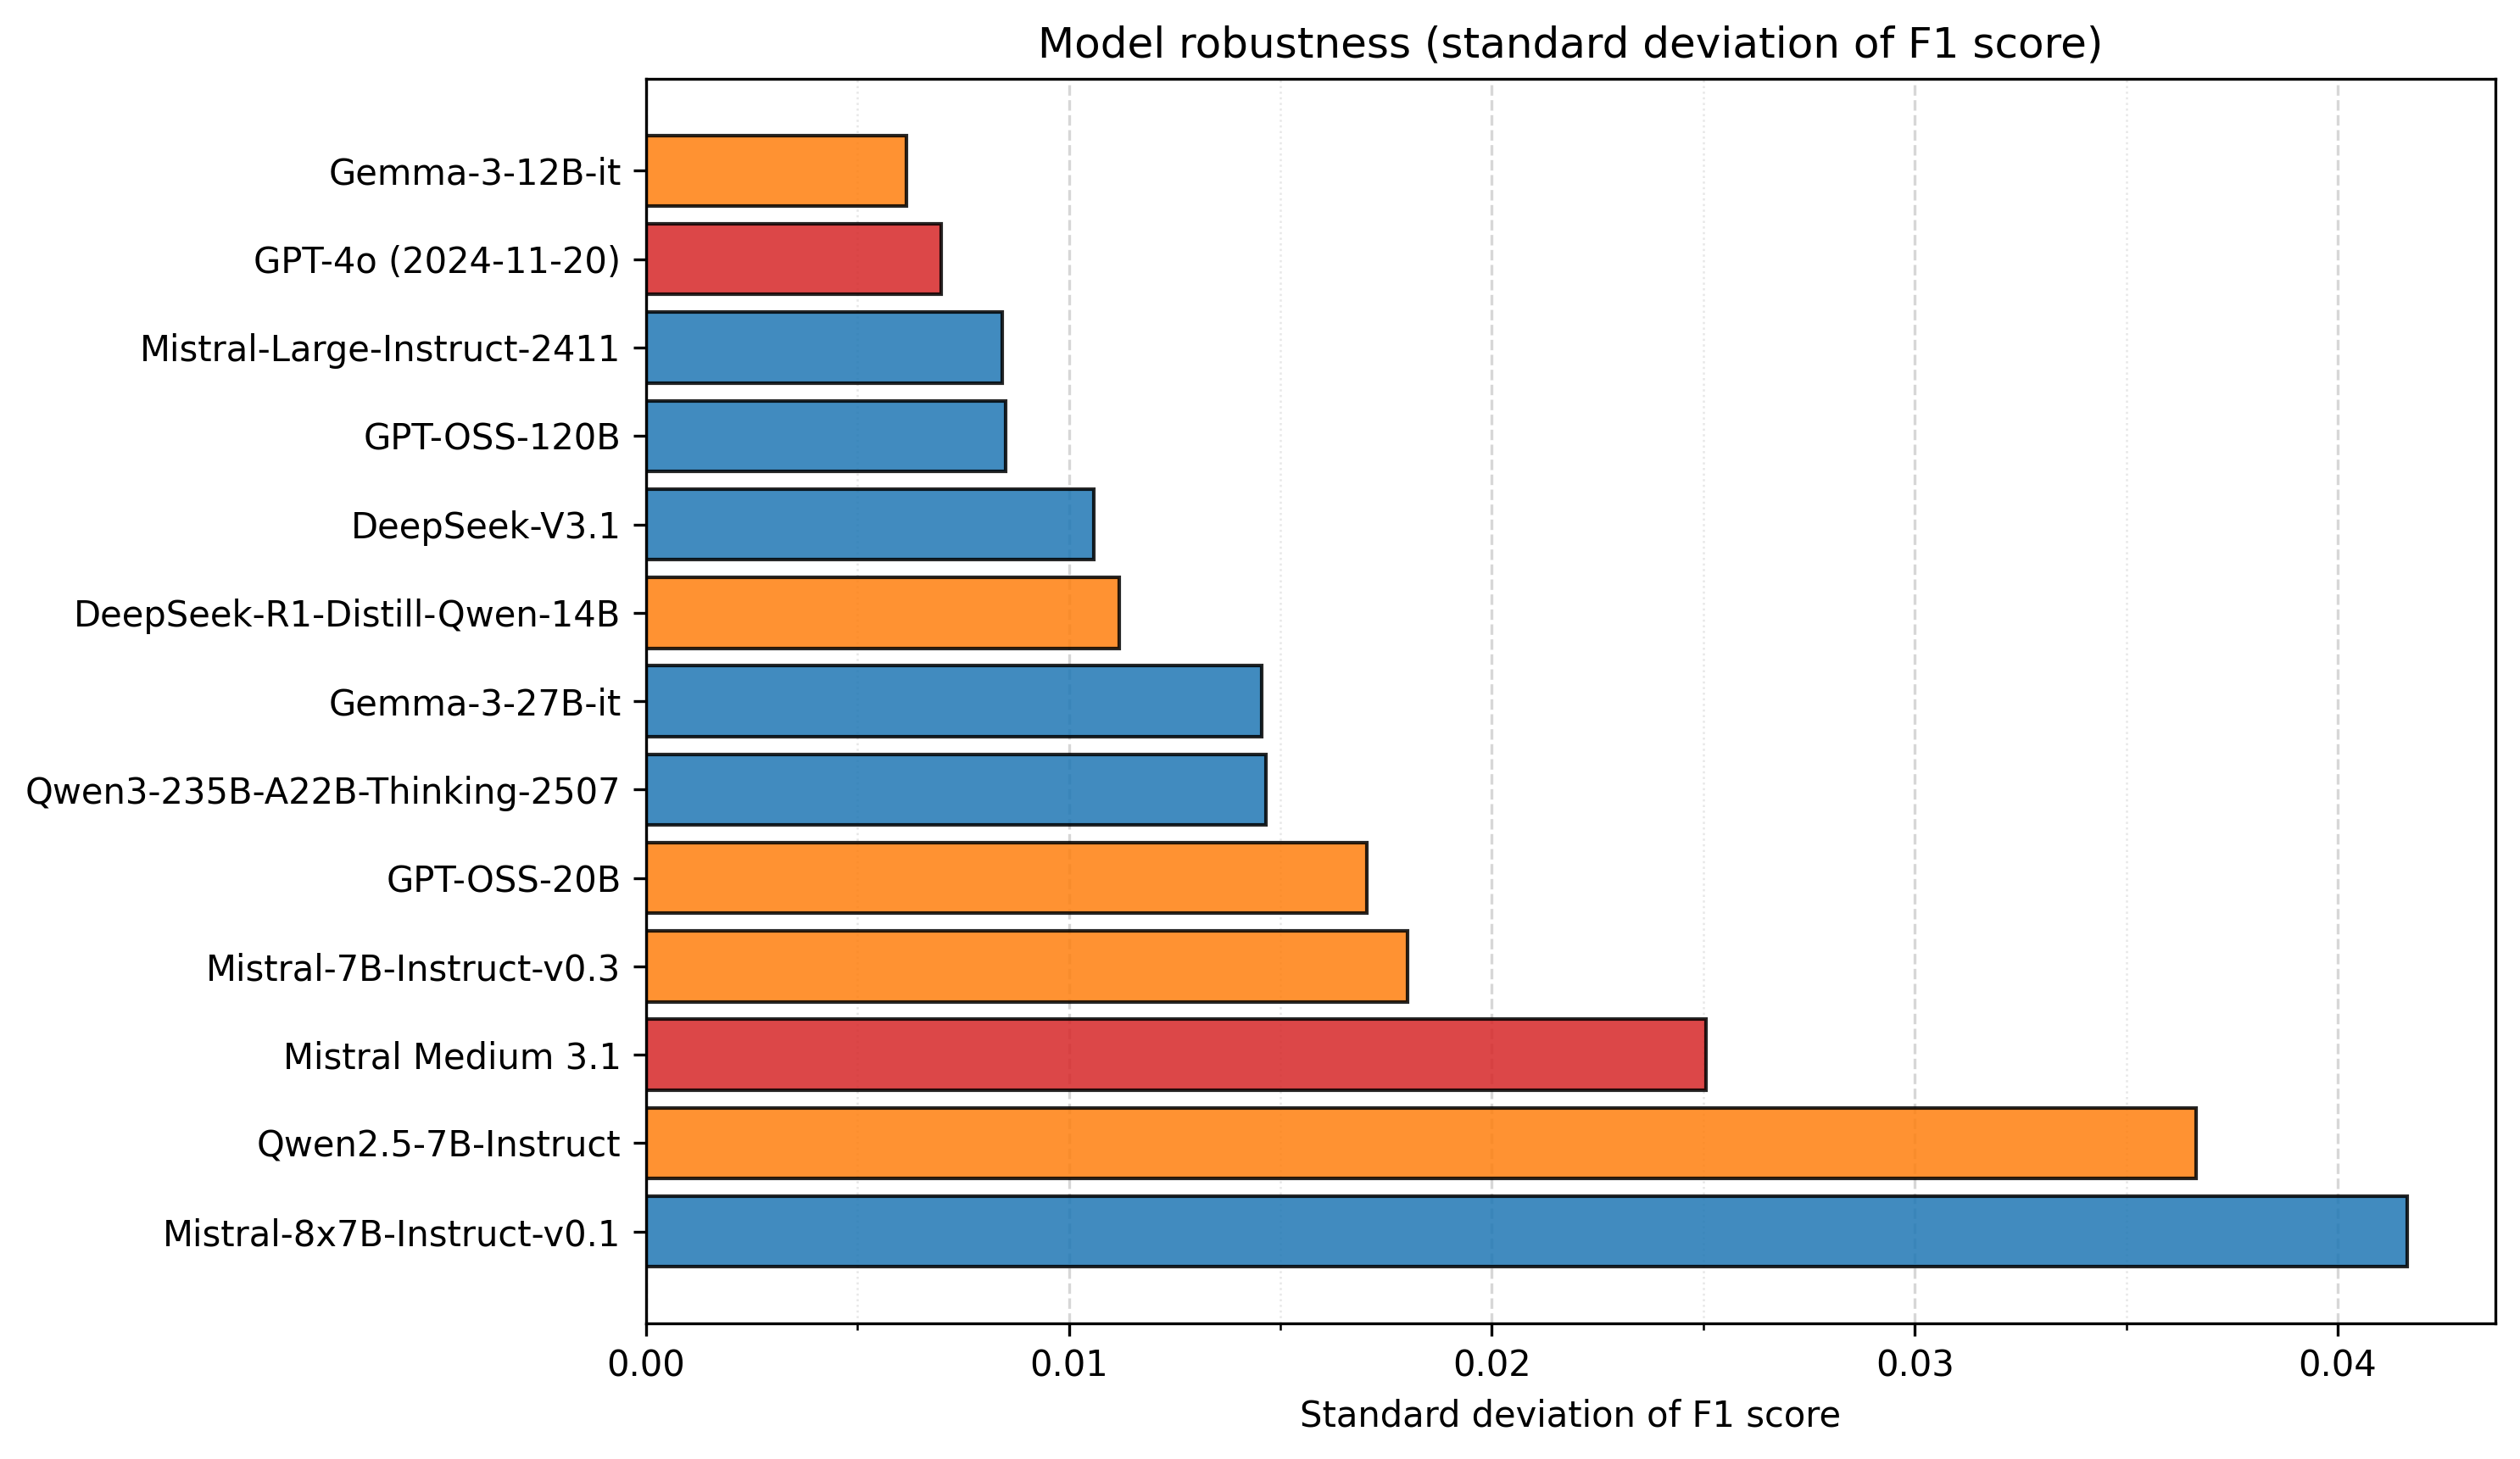
\includegraphics[width=0.7\textwidth]{images/results/evaluation_robustness_f1_std_en}
    \caption{Robustheit der Modelle gemessen an der Standardabweichung des F1-Scores über alle Wiederholungen hinweg.}
    \label{fig:results-evaluation-robustness-f1-std}
\end{figure}

Demgegenüber weisen \texttt{Mistral Medium 3.1}, \texttt{Qwen2.5-7B-Instruct} und vor allem \texttt{Mixtral-8x7B-Instruct-v0.1} mit Standardabweichungen zwischen $0{,}025$ und über $0{,}04$ eine deutlich höhere Varianz auf. Dies bedeutet, dass ihre Leistung stärker vom gewählten Seed abhängt, was die Vergleichbarkeit und Zuverlässigkeit verringert.

Neben der Varianz des F1-Scores ist auch entscheidend, wie oft das Modell nachgefragt werden muss, bis eine gültige JSON-Struktur zurückgegeben wird. Abbildung \ref{fig:results_evaluation_amount_of_retries} zeigt die durchschnittliche Anzahl notwendiger Retries pro Modell über 25 Testfälle. Die meisten Modelle lieferten bereits im ersten Versuch oder nach maximal einem zusätzlichen Aufruf eine korrekte Antwort. Hervorzuheben sind\linebreak~\texttt{DeepSeek-R1-Distill-Qwen-14B}, \texttt{GPT-4o}, \texttt{Gemma-3-12B-it} und \texttt{Mistral-\linebreak~Large-Instruct-2411}, die keinerlei Retries benötigten.

\begin{figure}[h]
    \centering
    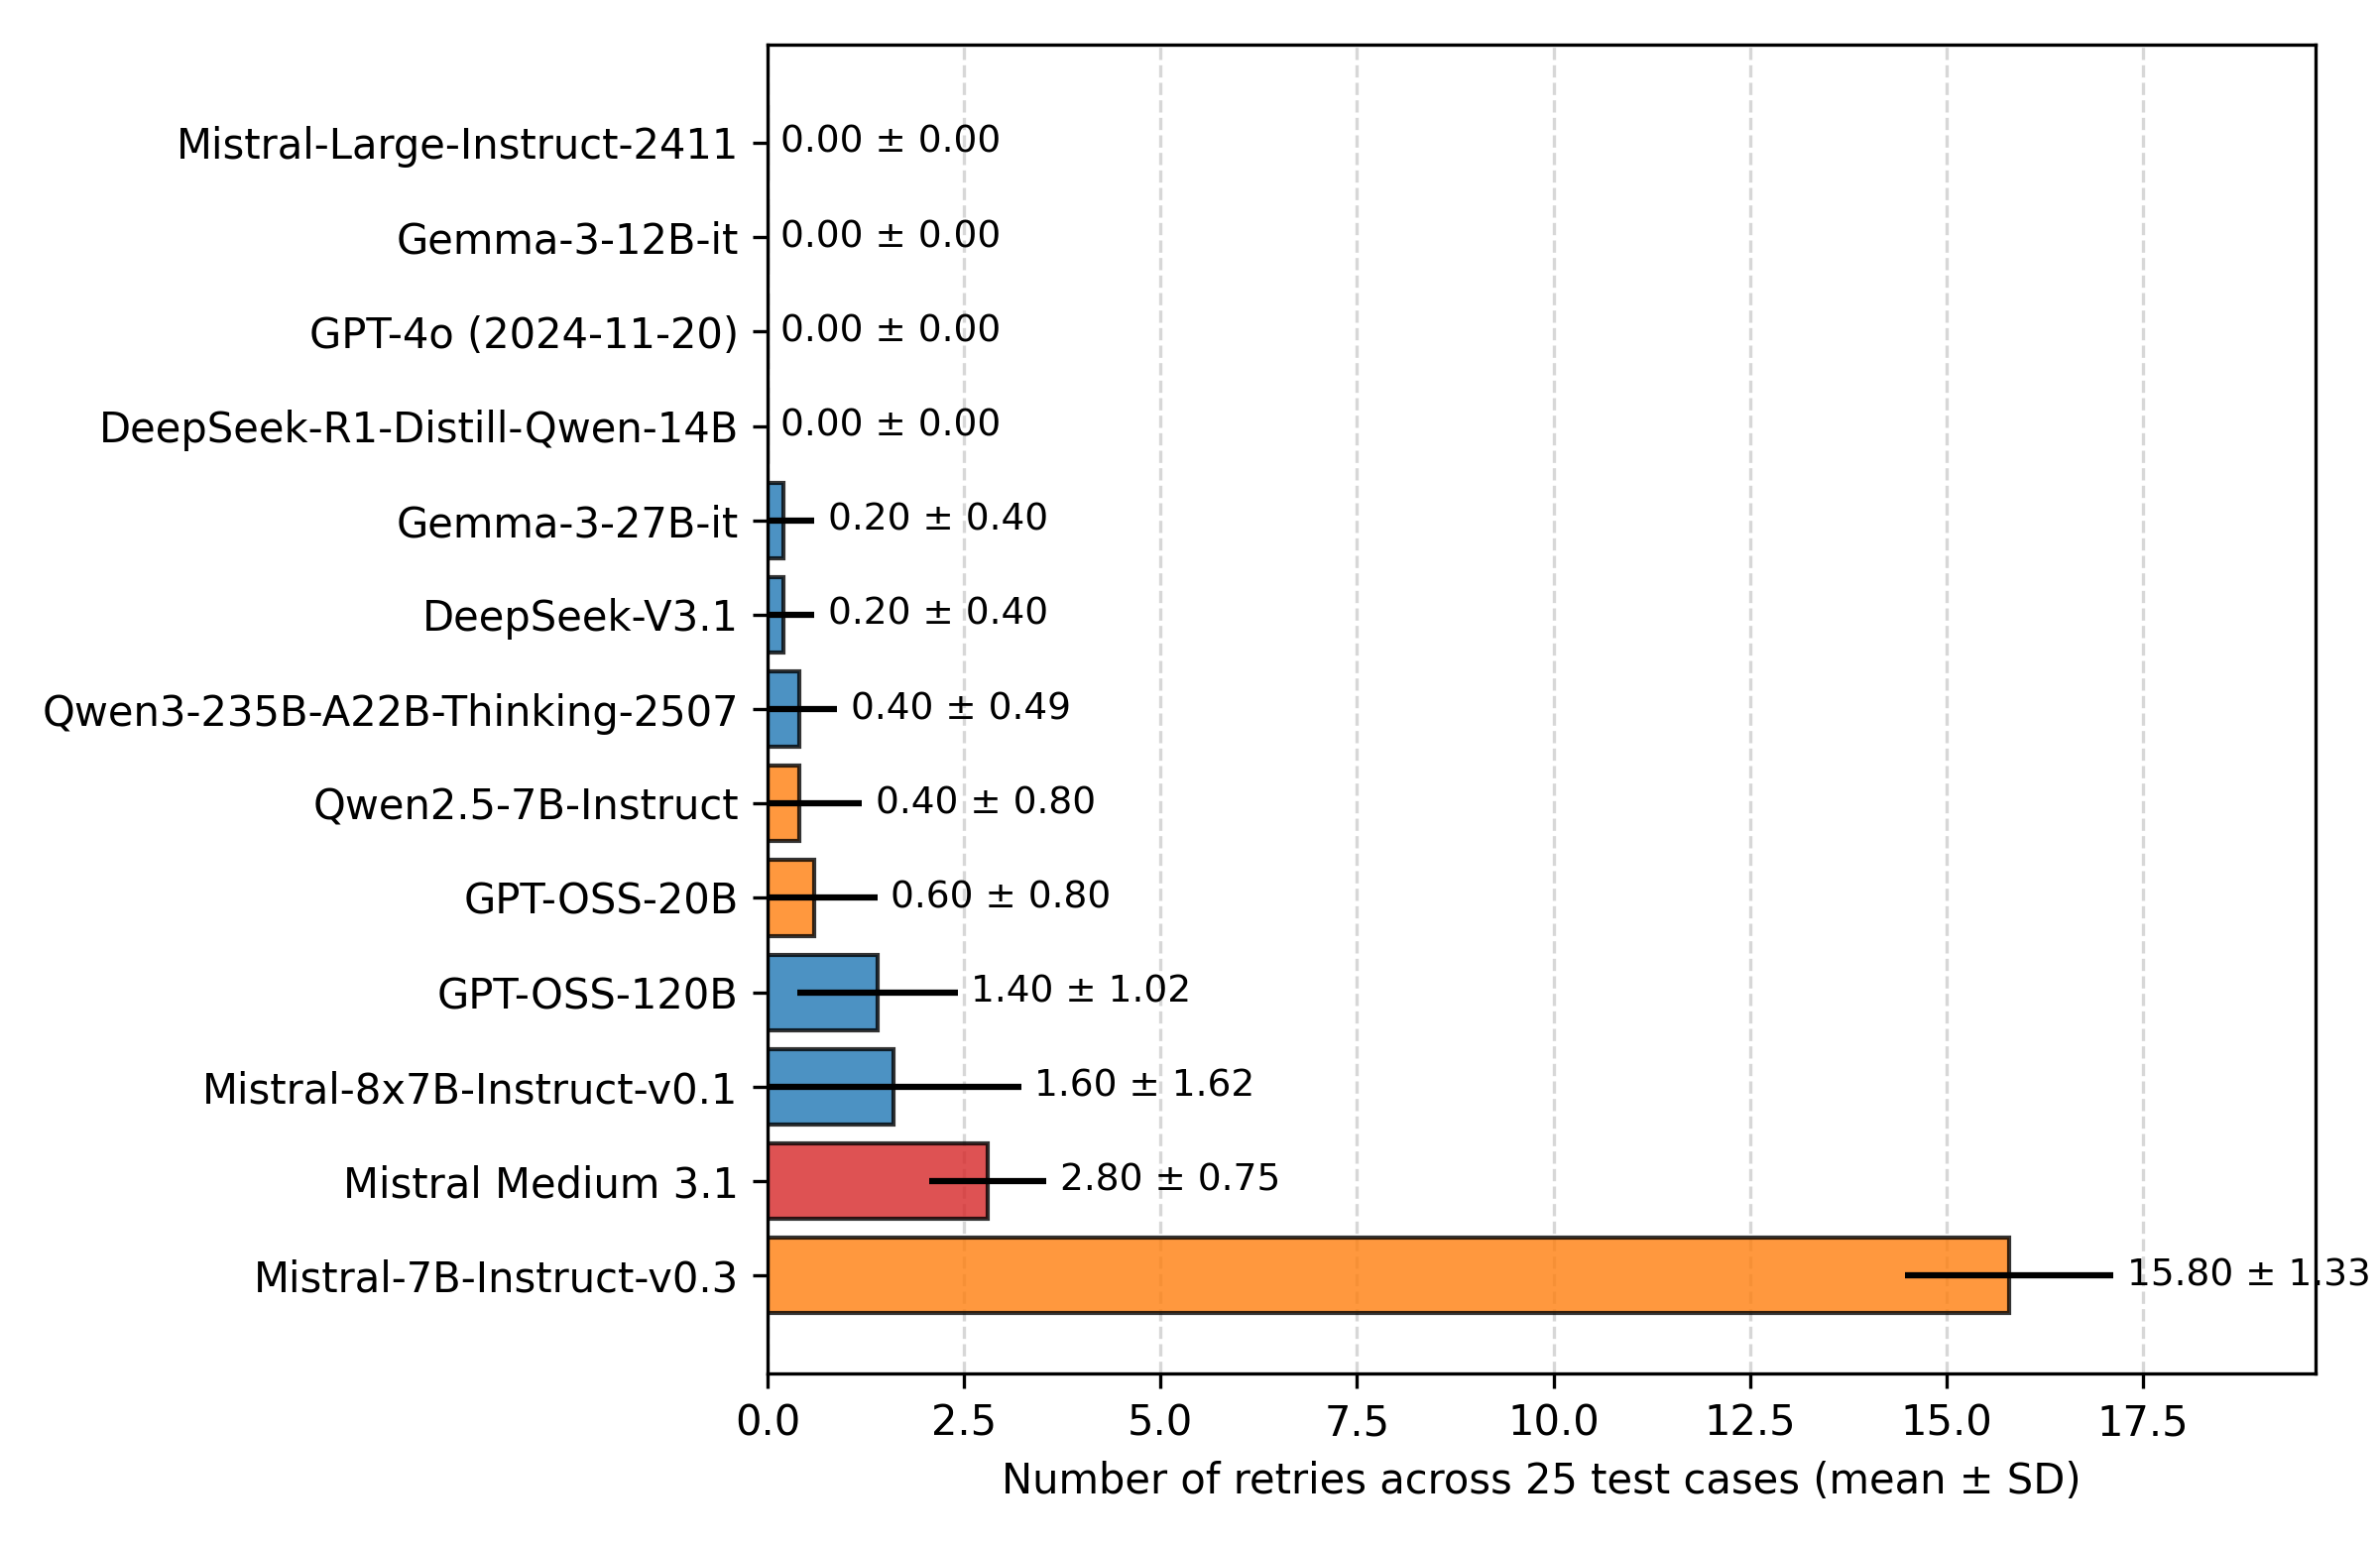
\includegraphics[width=0.7\textwidth]{images/results/evaluation_amount_of_retries_en}
    \caption{Durchschnittliche Anzahl der Retries, die notwendig waren, um für alle 25 Testfälle eine formatkorrekte JSON-Antwort zu erhalten.}
    \label{fig:results_evaluation_amount_of_retries}
\end{figure}

Am anderen Ende des Spektrums steht \texttt{Mistral-7B-Instruct-v0.3}, das im Mittel $15{,}8$ zusätzliche Aufrufe benötigte, was im Durchschnitt etwa $0{,}63$ Retries pro Testfall entspricht. Diese hohe Zahl verdeutlicht, dass das Modell Schwierigkeiten hat, die vorgegebenen Formatierungsregeln zuverlässig einzuhalten.

In Kombination mit der geringen Varianz sind \texttt{Gemma-3-12B-it}, \texttt{Mistral-Large-\linebreak~Instruct-2411} und \texttt{DeepSeek-R1-Distill-Qwen-14B} die robustesten Modelle: Sie liefern konsistente Ergebnisse und halten das Ausgabeschema zuverlässig ein. Modelle wie \texttt{Mistral Medium 3.1}, \texttt{Qwen2.5-7B-Instruct} und \texttt{Mixtral-8x7B-\linebreak~Instruct-v0.1} sind hingegen anfälliger für Schwankungen und erfordern häufiger Wiederholungen.
\section{Fehlerbilder und Grenzen}\label{sec:fehlerbilder-und-grenzen}

Die Fallstudien verdeutlichen zwei zentrale Schwachstellen. Erstens führen \emph{implizite Annahmen} zu konservativen, \ac{FP}-lastigen Entscheidungen, wenn entsprechende Hinweise im \ac{BPMN}-Modell nicht explizit modelliert sind. Das war beispielsweise bei der Anonymisierung von Klickraten im Testfall \enquote{Marketing-Kampagne} der Fall. Zweitens ist die \emph{Kontextverfolgung über Aktivitätsketten} nicht immer zuverlässig: Weiterverarbeitungen, die sich aus zuvor erhobenen Daten ergeben, werden vereinzelt nicht erkannt, was zu \ac{FN} führt. Dies zeigte sich etwa im Testfall \enquote{Route berechnen}, in dem personenbezogene Standortdaten aus einer vorherigen Aktivität an die Routenberechnung explizit weitergegeben wurden, ohne dass das Modell dies als kritisch erkannte. In der Praxis lassen sich daraus konkrete Gegenmaßnahmen ableiten: Zum einen sollten \ac{BPMN}-Modelle Datenflüsse sichtbarer machen, indem wichtige Elemente für den Kontext wie Datenobjekte/-speicher, Datenassoziationen, Nachrichtenflüsse, Annotationen sowie Pools/Lanes klar modelliert werden. Zum anderen sollten die Prompting-Strategien weiterentwickelt werden, um Modelle explizit auf die Bedeutung von Datenflüssen und Kontextinformationen hinzuweisen. Dazu zählt auch die Überprüfung, ob das Preprocessing der Klassifizierungspipeline ausreichend Kontext bereitstellt oder ob hier Anpassungen notwendig sind.

Die Generalisierbarkeit der Ergebnisse ist durch die Anzahl der Testfälle, deren Annotationen sowie die Auswahl der Modelle begrenzt. Zwar decken die 25 Testfälle eine breite Palette typischer \ac{DSGVO}-kritischer Szenarien ab, doch können sie nicht alle denkbaren Prozessvarianten und -kontexte repräsentieren. Künftige Studien sollten den Datensatz erweitern, um eine größere Vielfalt an Prozessen, Branchen und Komplexitätsgraden abzubilden. Dafür wurde in dieser Arbeit ein Labeling-Tool entwickelt. Zudem könnten weitere \acp{LLM} evaluiert werden, insbesondere solche mit neuen Architekturen oder Trainingsansätzen, um die Vergleichbarkeit zu erhöhen. Hinzu kommen technische Grenzen: Sehr große \ac{BPMN}-Prozesse können die Token-Limits der Modelle überschreiten, was eine Anpassung der Pipeline erfordern würde, etwa durch Prozesssegmentierung. Das Preprocessing verringert bereits die Token-Anzahl, doch sind weitere Optimierungen denkbar.

Schließlich werden die Ergebnisse durch die spezifischen Prompting-Strategien in der Klassifizierungspipeline beeinflusst. So ist etwa im genutzten System-Prompt verankert, dass die Klassifikation bei unklaren Aktivitäten eher konservativ ausfallen soll. Alternative Ansätze könnten zu unterschiedlichen Ergebnissen führen, vor allem mit Blick auf die Balance zwischen \ac{FP} und \ac{FN}. Künftige Arbeiten sollten verschiedene Prompting-Techniken und Pipeline-Designs vergleichen, um die bestmögliche Leistung zu erzielen. Die Leistungsbewertung könnte zudem domänenabhängig sein: In anderen Bereichen bestehen möglicherweise nicht so strenge Anforderungen an Recall und Precision wie im \ac{DSGVO}-Kontext. Abschließend ist zu betonen, dass die Klassifikation keine qualifizierte rechtliche Prüfung ersetzt, sondern als unterstützendes Werkzeug zur Risikominimierung dient.




